\documentclass[techrep,english]{ipsj} % techrep,

  \usepackage[nocompress]{cite}
  
  %\usepackage[dvips]{graphicx}
  \usepackage{latexsym}
  \usepackage[hyphens]{url}
  \Urlmuskip=0mu plus 1mu
  
  \usepackage{diagbox}
  
  \usepackage{tabu}
  \usepackage{footnote}
  \usepackage{tablefootnote}
  \usepackage{enumitem}
  \usepackage{times}
  \usepackage{float}
  \usepackage[binary-units=true,quotient-mode=fraction,table-auto-round]{siunitx}
  \sisetup{detect-all}
  \sisetup{range-phrase=--}
  \sisetup{range-units=single}
  \DeclareSIUnit\years{years}
  \usepackage{graphicx}
  \usepackage{subfigure}
  \usepackage{amsmath,amsfonts,amssymb}
  \usepackage{comment}
  \usepackage{multirow}
  \usepackage{bbding}
  \newcommand{\tabincell}[2]{\begin{tabular}{@{}#1@{}}#2\end{tabular}}
  \usepackage{times}
  \usepackage{soul}
  \usepackage{color}
  \usepackage{latexsym}
  \usepackage{booktabs,multirow,multicol}
  \usepackage{todonotes}
  \usepackage{multirow}
  \usepackage{comment}
  \usepackage{tabularx}
  \usepackage{url}
  
  \def\Underline{\setbox0\hbox\bgroup\let\\\endUnderline}
  \def\endUnderline{\vphantom{y}\egroup\smash{\underline{\box0}}\\}
  \def\|{\verb|}

\graphicspath{
    {resources/}
}


%\def\Underline{\setbox0\hbox\bgroup\let\\\endUnderline}
%\def\endUnderline{\vphantom{y}\egroup\smash{\underline{\box0}}\\}
%\def\|{\verb|}

\setcounter{volume}{26} % vol21=2013, 22=14, 23=15, 24=16, 25=17, 26=18
\setcounter{number}{1}
\setcounter{page}{1}

\usepackage[varg]{txfonts}%%!!
\makeatletter%
\input{ot1txtt.fd}
\makeatother%

\usepackage[hidelinks]{hyperref}
\usepackage[nameinlink,noabbrev,capitalise]{cleveref}

\begin{document}

\title{Towards Accelerating Deep Neural Network Training on FPGAs Facilitating the Use of Variable Precision}

\affiliate{Riken}{RIKEN Center for Computational Science, Chuo-ku, Kobe, Hyogo 650-0047 Japan}
\affiliate{TiTech}{Tokyo Institute of Technology, 
Meguro, Tokyo 152--8550, Japan}
\affiliate{TUDelft}{Delft University of Technology, Mekelweg 2, 2628 CD Delft, Netherlands}

\author{Erwin de Haan}{TiTech,TUDelft}[e.r.dehaan@student.tudelft.nl]
\author{Artur Podobas}{TiTech}[podobas.a.aa@m.titech.ac.jp]
\author{Satoshi Matsuoka}{Riken,TiTech}[matsu@is.titech.ac.jp]

\begin{abstract}
The race for larger and deeper neural networks are leading researchers, vendors and practitioners to re-think architectural design decisions taken decades ago in hope to improve performance.
Among these decisions, reducing the numerical format is thought to be one of prime candidates to increasing performance.
Unfortunately, modern hardware has limited support for this, and the impact of modifying floating-point formats and its size remains shrouded in mystery.
To help investigate what the effects of varying the precision during deep-learning training are, first an architecture using reconfigurable hardware needs to be developed.
Through this work, we seek to accelerate arbitrary precision deep-learning training using Field-Programmable Gate-Arrays by leveraging Intel FPGA SDK for OpenCL.
Preliminary results show promise for implementations based on precisions or number formats that currently only have low performing implementations on conventional CPU and GPU hardware.
\end{abstract}

%\begin{keyword}
%Journal of Information Processing, \LaTeX, style files, ``Dos and
% Don'ts'' list
%\end{keyword}

\maketitle

\section{Introduction}
The present paper describes our efforts toward a customized and generalized framework for design-space exploration using alternative numerical floating-point formats through FPGAs.

The recent explosion in artificial intelligence – in particular that of deep neural networks based on back-propagation – has triggered a storm in the introduction and creation of specialized compute devices.
Commercial platforms such as Microsoft’s BrainWave~\cite{msbrainwave}, Google’s TPUs~\cite{googletpu}, and Fujitsu’s DLU~\cite{fujitsudlu} are all examples of specialized circuitry dedicated to low-power, high-performance Deep-Learning (DL) training and/or inference.
Meanwhile, existing general-purpose manufacturers are empowering their architecture with custom floating-point units that trade precision for performance, such as Intel’s Knights-Mill~\cite{knm} and NVIDIA’s Volta-100~\cite{volta100}.
It is clear that Artificial Intelligence and Deep-Learning will have a prioritized presence in modern architecture -- today and in the near future.

In the pursuit for faster and more energy efficient deep-learning architecture, there is a need to critically review long-standing architectural design decisions taken by computer architects decades ago.
One of the oldest design decision concerns the representation of real-valued numbers, otherwise known as the floating-point representation.
The IEEE-754 floating-point representation is one of the few relics that remain unchanged in computing today.
Reducing the size of the floating-point representation can have dramatic (and positive) impacts on the performance: more compute per unit silicon, more compute per unit bandwidth, and lower power consumption.
Several alternatives to the IEEE-754 format are indeed emerging, such as Microsoft’s Deep-Learning format~\cite{msbrainwave}, Intel’s FlexPoint~\cite{intelflexpoint}, Google’s custom TPU format~\cite{tpuformat}, and Posits~\cite{posits}.

However, exploring the space around IEEE-754 floating-point representations and its alternatives pose a significant engineering problem: hardware and software infrastructure is to tightly coupled to the IEEE-754 standard that changing any part of it incurs a high engineering overhead.
One alternative is to simulate alternative floating-point representations in software, for example using soft-float or MPFR libraries~\cite{softfloat}, but the resulting performance is often several magnitudes lower than hardware implementations, limiting the size of the study conducted.
Furthermore, simulating alternative numerical formats in software are incapable of using any compiler optimizations, nor can they leverage the vector instruction often crucial to reach application performance in modern processors.
Porting the full software infrastructure stack is possible (and inevitable), but is a non-trivial effort that requires changes to the compiler, standard libraries and (possibly) the Application-Binary-Interface (e.g.\ calling convention).

A better way to explore floating-point representation is to leverage Field-Programmable Gate-Arrays (FPGAs).
An FPGA is a device consisting of several millions re-programmable look-up tables (LUTs) that together with programmable routers give a very malleable silicon substrate second only in performance to Application-Specific Integrate Circuits (ASICs).
Modern FPGAs can be clocked at several hundreds MHz, and contain enough compute to rival even Graphics-Processing Units (GPUs), making them ideal to study architectural design choices.
Furthermore, with the recent growth in popularity of High-Level Synthesis (HLS) tools, programming these devices can be as simple as writing C/C++ code, and delegate the software-to-hardware transformation effort to the compiler.

We contribute with the following:
\begin{itemize}
\item Proposed design for a generalized FPGA training architecture targeting variable numerical formats, and
\item Evaluation and analysis of core computation patterns, including FPGA resource utilization
\end{itemize}

The remainder of our paper is structure in the following way: \cref{sec:relwork} positions our work against other, similar efforts.
\cref{sec:framework} gives a background to machine learning and FPGAs, and describes our proposed architecture.
\cref{sec:method} overviews our experimental methodology, and is followed by our preliminary results in \cref{sec:result}.
We conclude in \cref{sec:conclusion}.

\section{Related Work}\label{sec:relwork}
Field-Programmable Gate-Arrays (FPGAs) have extensively been used to probe and explore various architectural design decision, including those of deep-learning.
The large majority of existing work limit themselves to inference, primarily due to the simpler design layout (little intermediate data needs storing).
Levering FPGAs have allowed researchers to decrease the number of bits allocate to the numerical representation, going as far as inferring popular networks such as  AlexNET~\cite{krizhevsky2012imagenet} using as few as binary~\cite{shimoda2017all,umuroglu2017finn} (1-bit) weights.
Inferring networks that uses few bits to represents weights (called Quantized Neural Networks~\cite{courbariaux2016binarized}) requires subtle yet necessary changes to the training phase~\cite{binaryconnect,courbariaux2016binarized,zhou2016dorefa}.
Lately, modern deep-learning framework are having support for reduced precision training, some driven by leading FPGA vendors such as Xilinx~\cite{xilinxml}.
Dicecco et al.~\cite{dicecco2017fpga} are working on a framework similar to ours that trains neural networks using FPGAs while modifying the numerical format.
Their work primary focus on the IEEE-754 format and convolution layers where-as we aspire to include alternative format such as posits~\cite{posits}.
Using posits in deep-learning was intended the focus of Langroudi et al.~\cite{langroudi2018deep}’s work; however, they only compared the performance against fixed-point and only \textit{stored} the weights as posit (the computation was still done using IEEE-754).

FPGAs are not unique to vary the numerical precision of deep neural networks, and several ASICs have been produced for quantized neural networks.
Most of these focus only on inference (for embedded deployment)  for low-power embedded domains; these include YodaNN~\cite{yodann}, BinaryEYE~\cite{binaryeye} and ChipMunk~\cite{chipmunk}; these ASICs were shown to consume up-to two magnitudes low power compared to similar FPGA solutions.

Commercially most vendors do support some form of reduced precision mode.
Intel’s Knight’s Mill~\cite{knm} architecture replaces one of the AVX-512 vector units of Knight’s Landing with a Vector Neural Network Instruction (VNNI) unit, capable of performing dot-products in a mixed IEEE-754 16-bit and 32-bit mode.
A similar process (reduced precision multiplication, full precision accumulation) is also applied in NVIDIA’s Volta-100 line GPUs.
These mixed-precision units drastically improve the Artificial-Intelligence compute capabilities (AI-FLOPs) of modern systems, trading silicon resource for increased compute with arguable small impact on training performance.
Vendors also embrace drastically different formats, notably in Intel’s NERVANA~\cite{nervana} (likely where FlexPoint~\cite{intelflexpoint} is used) and Google’s TPU~\cite{tpuformat} (which have more bits in the exponent compared to the mantissa).


\section{A FPGA-based NN Framework}\label{sec:framework}
\subsection{Field-Programmable Gate-Arrays}

FPGAs can be used for a great variety of things, from accelerating computational algorithms to implementing a hardware design before taping out full chip.
They are devices that can represent reconfigurable hardware.
A normal FPGA work-flow consists of writing in a hardware description language.
Then synthesizing the design and finally placing and routing the design.
This is a lengthy process and complex designs in hardware description languages are hard to maintain.
In this work we will focus on using the OpenCL interface to the FPGA.
OpenCL is a framework specified by the Khronos Group\footnote{Specification available at: \url{https://www.khronos.org/opencl/}} in 2009, to work with all kinds of processors, accelerators and other heterogenous compute devices, in recent years the FPGA vendors have made efforts to make it easier to leverage FPGA resources by computer scientists and not only hardware designers.
So OpenCL is one of the ways to leverage high level synthesis.
High level synthesis take a design specification in a high level language like C or in this case the modified version of C99 that is used for OpenCL kernels.
And the synthesizer makes an RTL design description from this design automatically after which the normal work-flow is resumed.

FPGAs are made up of a reconfigurable fabric.
The fabric they are made up of consists of vast arrays of switches and other routing hardware to connect all the functional elements, like multipliers, block RAMs and LUTs, in any way possible.
The LUTs can be used to implement any mathematical function, like addition, multiplication, boolean functions and more.
This makes them very suitable for the research described in this paper.
It gives total freedom to design a hardware implementation to explore algorithms in a hardware setting without having to resort to software simulations and the performance limitations that follow from that.

\begin{figure}[ht]
  \centering
  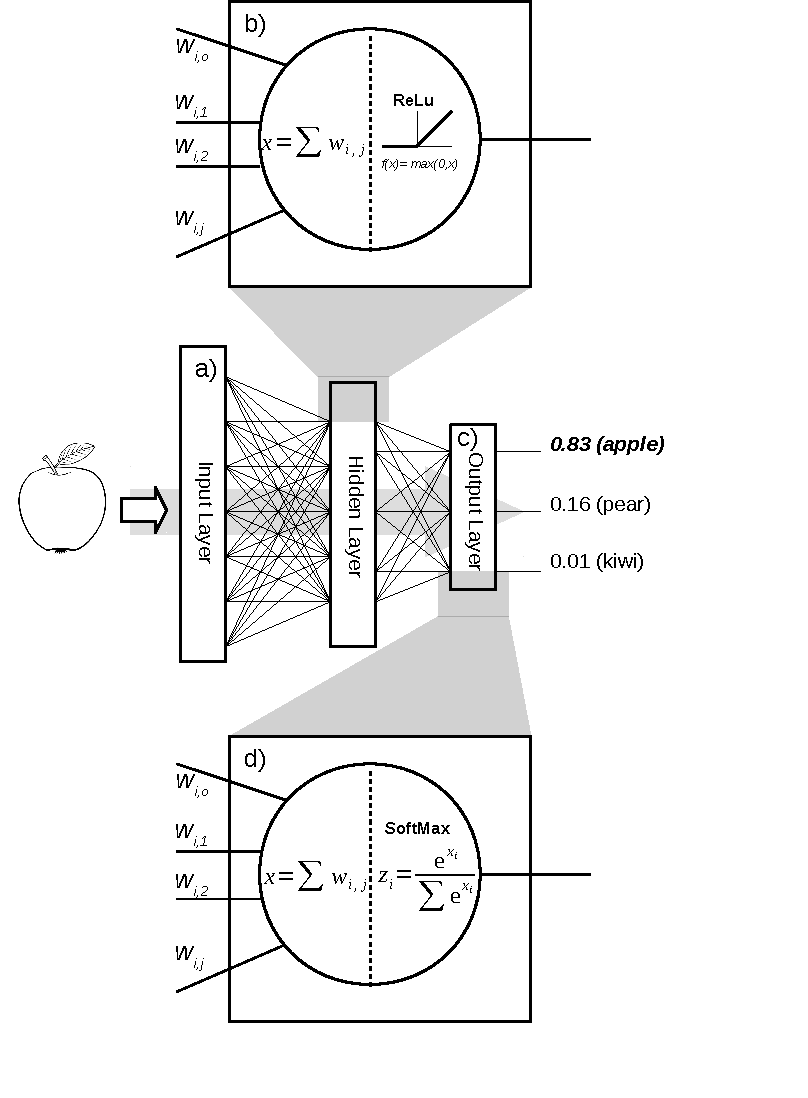
\includegraphics[width=\linewidth]{example_ann-crop.pdf}
  \caption{The basics of artificial ``deep'' neural networks, showing the input (a) layer, the hidden (b) layer, and the output (c-d) layer.}\label{fig:ann-example}
\end{figure}

\subsection{Neural Networks}
An Artificial Neural Network (ANNs) is a system inspired by the biological nervous system-- a system built around the concepts of \textit{neuron}s as the main computational agents.
\Cref{fig:ann-example} illustrates an example of a typical “deep” neural network: a network that consists of a input layer, and output layer, and a number of \textit{hidden} layers in-between.
The number of hidden layers in modern neural networks can be very large: AlexNet (2012)~\cite{krizhevsky2012imagenet} has eight, VGG16 (2014)~\cite{simonyan2014very} has 16 layers, GoogleNet (2014)~\cite{szegedy2015going} has 22 layers, and ResNet (2016)~\cite{he2016deep} has 152 layers.
The trend seem to favor larger and deeper neural networks.
The input layer of a neural network (in our example, a classifier) contains the (possibly pre-processed) inputs, such as images (for image recognition), words (in natural language processing), or motifs (in graph processing).
In our humble example, the input is an image of an apple, where each pixel has an all-to-all connection to the hidden layer-- a so-called \textit{dense} layer. The dense-layer (or fully-connected layer) is the most basic of all layers, and nearly all (e.g.\ convolution) layers are derived from it.
Each layers consists of a number of \textit{neurons} – the main compute agent of the network.
Each edge that connect to a particular neuron is called a \textit{synapse}, and comes with a \textit{weight} (\(w_{i,j}\)) in the figure, where \(i\) is the index of the neuron).
The neuron integrates the weights (\cref{fig:ann-example}:b) of all input synapses, adds a local bias, and applies a activation function to compute the output of the neuron. The activation function varies between networks, but commonly used activation functions include: the sigmoid (\(f(x) = \frac{1}{1+e^{-x}}\)), the rectifier (ReLu, \(f(x) = max(0,x)\)), or hyperbolic tangent (\(f(x) = tanh(x)\)).
In \cref{fig:ann-example}:b (and commonly in image processing network), the simple and compute-\textit{in}expensive ReLu activation function is used in the hidden-layers of the network. The final layer of our classifier neural network is an output layer, \cref{fig:ann-example}:c. In the output layer, the activation function is often a \textit{softmax} (\cref{fig:ann-example}:d), which scales all outputs such that their sum equals one.

Inferring (predicting) using a deep neural network is done by connecting the input to what is to be predicted, and sequentially activating each layer --from the front to the back of the network-- and propagating the output of each layer into the next.
This effort is called \textit{forward propagation}. Training the network is done in a similar but reverse fashion -- errors are calculated at the output and propagated backwards.
At this point in time, our framework focuses on forward propagation.

\begin{figure*}[p]
  \centering
  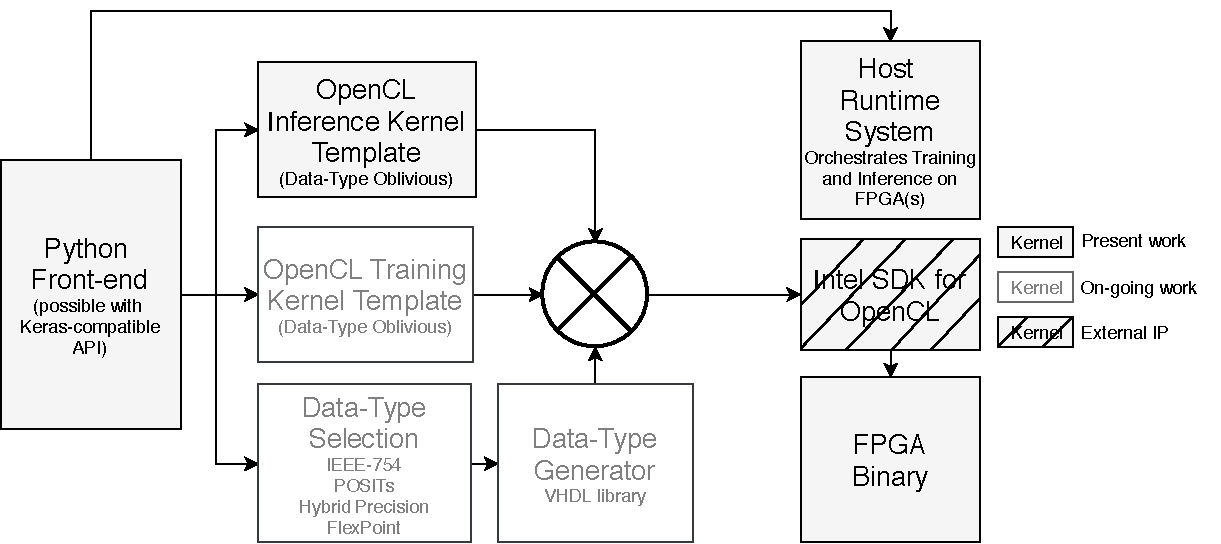
\includegraphics[width=0.7\linewidth]{training_overview.pdf}
  \caption{Overview over our framework, showing blocks existing (black) and components currently worked on (gray).}\label{fig:overview}
\end{figure*}

\subsection{FPGA Neural Network Framework}
We aspire to create a neural network framework that allows design-space exploration with different numerical data formats.
Our framework, illustrated in \cref{fig:overview}, consists of a number of components.
We have chosen to rely on Python as the high-level frontend for our framework.
It is through python that a user create a networks, selects inputs, and decides what data formats to use.
Once a particular configuration is selected, our framework generates data-type oblivious training and inference code that targets Intel's OpenCL SDK for FPGAs.
By data-type oblivious we mean that all operations associated with any particular data-type representation remain unresolved at the point of creation, as they will not depend on any of the native data-types or functionality of the OpenCL language.
Instead, our Python framework invokes a Data-type selector, which automatically generates a low-level hardware description language (HDL) library that contain commonly used operators for the selected data-type.
Once the Register-Transfer Level (RTL) library has been generated, it is merged with the data-type oblivious OpenCL template to yield the final description, which now can be synthesized using EDA tools and used.
Invisible to the user, our host runtime system handles all communication, invocation and control over the FPGA from the host side.

The present paper focuses on the IEEE-754 part of inference, where training and alternative data-types are on-going and future work.

\subsubsection{Design overview}
\Cref{fig:block-diagram} shows a overview of the system.
The backwards kernels are a work in progress, so for now we use an external training script.
The backwards kernels are the kernels that calculate the error and back propagate the error while updating the weights and biases in the network used during training.
During inference the host code, written in python, does one forward kernel call for every layer.
And does a final softmax kernel call to get the final prediction.
For performance this could obviously be done on the host, given the limited size of most final layers, but performance is not the main goal of this effort.
The main goal to make replacing the numerical format easier, and thus all the calculations need to be done in that format, and an FPGA is better at accommodating that without a huge performance impact.

\begin{figure*}[p]
  \centering
  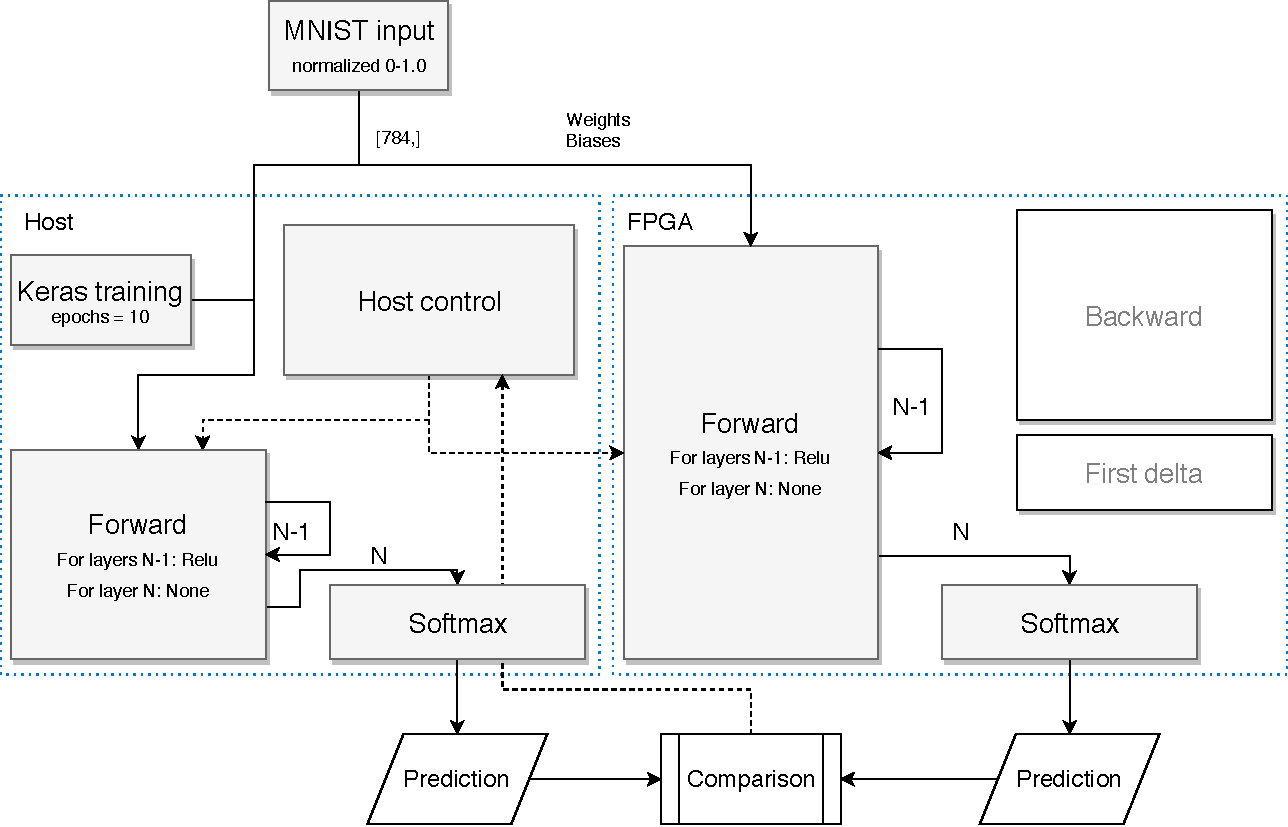
\includegraphics[width=0.7\linewidth]{block-diagram.pdf}
  \caption{Block diagram of the implementation, on the left the host code, and on the right side the device code. The host side orchestrates all the computation on the device side.}\label{fig:block-diagram}
\end{figure*}

\begin{figure*}[p]
  \centering
  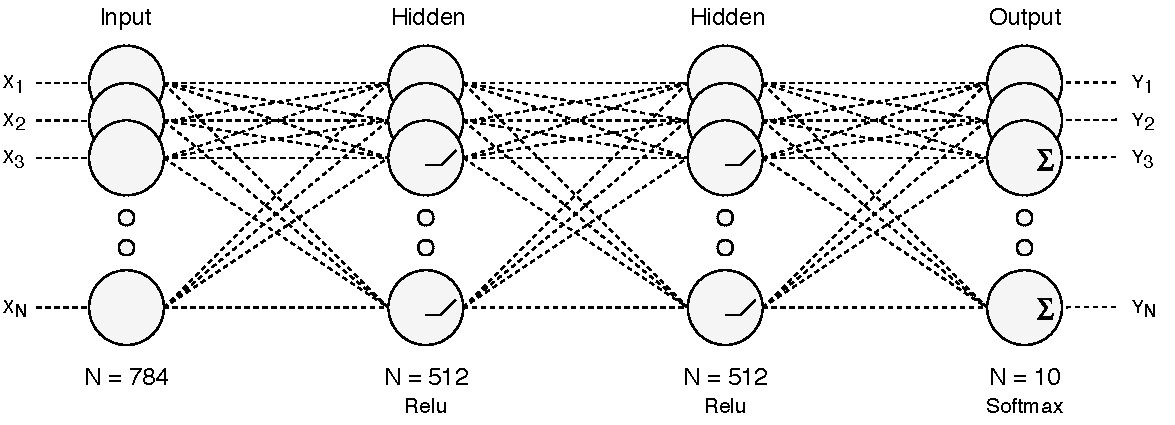
\includegraphics[width=0.6\linewidth]{mnist-network.pdf}
  \caption{MNIST sample network configuration}\label{fig:mnist-network}
\end{figure*}
\begin{figure*}[p]
  \centering
  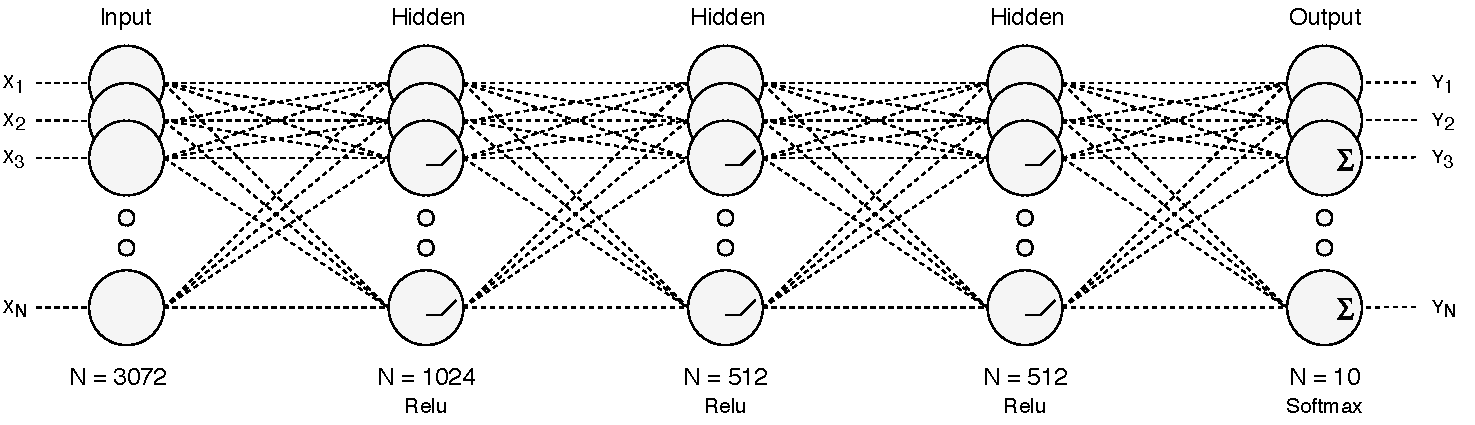
\includegraphics[width=0.8\linewidth]{cifar10-network.pdf}
  \caption{CIFAR-10 sample network configuration}\label{fig:cifar10-network}
\end{figure*}

\subsubsection{Design details}
All weight matrices are transposed in memory, this to optimized the memory access pattern of the matrix-matrix multiplication.
The main inference is done using an blocking implementation of the matrix multiplication.
So a block is fetched from the activations and the weights and placed in the block RAM on the FPGA.
The computation result is also stored on the block RAM, before a routine writes it back to global memory.
The block RAM has a much lower latency than the global memory.
This speeds up throughput by a large margin.
Block RAM is equivalent to the shared or local memory of contemporary GPUs.

The OpenCL SDK from Intel used for this design, tries to pipeline loops in single work item kernels, as opposed to NDRange kernels. % Reference to Intel OpenCL Manual?
To get maximum performance the aim is to get an initiation interval of one.
That is to say that a new loop iteration is scheduled every clock cycle.
To get this to work on the inner most loop, one that is essentially a reduction.
An array is used to store all output in separate locations, this way the loop can be fully unrolled.
For the containing loops, serial dependencies are to be avoided whenever possible.
So different loop iterations are fully data-independent.
For the outermost loop that processes one block this behavior is not possible, since the output block is written to multiple times.
If there was enough space on the FPGA theoretically multiple blocks would be able to be processed in parallel.
In the future the training kernel also needs to fit, so it was decided not to try parallelize this further.

\subsubsection{Design decisions}
One of the main choices with the largest effect on implementation is whenever to keep all weight matrices in memory transposed.
During inference this is very beneficial, as this makes most reads sequential.
In early stages of development it sped up the kernel performance by a factor of \num{3}.
During training, using stochastic gradient descent, this can be a problem though, the weight matrix should now be transposed back for the most efficient memory access patterns.
But since the arithmetic density of the training process is higher, the effect might be slightly less pronounced.
An other decision was to take the most outer loop, the loop over all the layers, to the host.
This loop can not be pipelined since there is serial dependency, so it makes more sense execute this loop on the host CPU.
This both saves space on the FPGA and it simplifies the generated hardware.

\section{Methodology}\label{sec:method}
\subsection{Experimental Platform}
The software versions and hardware configuration are shown in respectively \cref{tab:software-versions} and \cref{tab:test-hardware}.
All kernels were compiled with \texttt{-O3 -fp-relaxed}.
\texttt{-fp-relaxed} gives the compiler some more freedom with the order of operations, this gives about a \SIrange{10}{15}{\percent} performance benefit.% without changing the numerical output.
\begin{table}[h]
  \centering
  \caption{Used software versions}\label{tab:software-versions}
  \begin{tabular}{ll}
    \toprule
    \textbf{Software} & \textbf{Version} \\
    \midrule
    Python & v3.6.3 \\
    Keras & v2.2.0 \\
    TensorFlow & v1.8.0 \\
    Intel Quartus & v17.1.0 \\
    Intel OpenCL & v1.1 \\
    \bottomrule
  \end{tabular}
\end{table}
\begin{table}[h]
  \centering
  \caption{Test hardware}\label{tab:test-hardware}
  \begin{tabular}{ll}
    \toprule
    \textbf{Hardware} & \textbf{Configuration} \\
    \midrule
    Intel i7-3930K & \SI{3.20}{\giga\hertz} \\
    DDR3 RAM & \SI{1333}{\mega\hertz} Dual Channel \\
    Arria 10 ($\times$1) & Nallatech 510T \\
    \bottomrule
  \end{tabular}
\end{table}

\subsection{Network Tested + Data-set}

The used example networks are multi-layer perceptron (MLP).
So all layers are an array of neurons and every neuron is connected to every neuron in the next layer.
These layers are often called ``Dense'' layers.
The first data set used was MNIST~\cite{lecun2010mnist}, MNIST is a collection of 28\(\times\)28 gray scale images of hand written arabic numerals.
So the data set provides \num{784} input features.
The structure of the sample MNIST network is shown in \cref{fig:mnist-network}.
In total a three layer network plus the input layer, or three sets of weight matrices and bias vectors.
The data set was trained using the first \num{60000} images from the MNIST data set.
The last \num{10000} images are used as the test data set.\\
The second data set used was CIFAR-10~\cite{krizhevsky2014cifar}, so \num{3072} input features.
The structure of the sample CIFAR-10 network is shown in \cref{fig:cifar10-network}.\\
The data set was trained using the first \num{50000} images from the data set.
The last \num{10000} images were used as the test data set.
All training was done using a batch size of \num{128}.
The CPU code was implemented using the NumPy array.dot function.

\section{Results}\label{sec:result}
The host (NumPy based) code benchmarked at \num{60} GFLOPS for straight-forward inference of the first network and about \num{160} GFLOPS for the second network.
A first naive implementation on the FPGA clocked about \num{2.5} GFLOPS for this problem size.
Transposing the weight matrix sped up the kernel to around \num{7.5} GFLOPS.\@
The results for the different final FPGA kernels are shown in \cref{tab:kernel-performance}.

\begin{table}[h]
  \centering
  \caption{FPGA Kernel performance}\label{tab:kernel-performance}
  \begin{tabular}{llll}
    \toprule
    \textbf{Block size} & \textbf{GFLOPS MNIST}  & \textbf{GFLOPS CIFAR-10}  \\
    \midrule
    64$\times$64 & \num{17.8} & \num{18.9}  \\ % kernel_nn_blocking_B64inorder_hw_2018-06-28T22.52.27.aocx Network MNIST: [28 * 28, 512, 512, 10] CIFAR: [32 * 32 * 3, 1024, 512, 512, 10]
    16$\times$16 & \num{4.3} & \num{4.4} \\ % kernel_nn_blocking_B16inorder_hw_2018-06-28T22.53.27.aocx Network MNIST: [28 * 28, 512, 512, 10] CIFAR: [32 * 32 * 3, 1024, 512, 512, 10]
    \bottomrule
  \end{tabular}
\end{table}

The performance is memory bandwidth limited for these kernels.

\subsection{FPGA Resource Utilization}
The kernel resource utilization is shown in \cref{tab:fpga-util}.
The main limiting factor is the available block RAM.
To stop the calculation of extra padding lines in the matrices, the block size should be a multiple of most of the layer sizes.
Larger block sizes would exhaust the block RAM on the used FPGA device.
The next logical size up from \num{64} would be \num{84} (\num{3}\(\times\)\num{28}), this would use to much of the block RAM already.
This is because there are three block buffers and the relationship between block size and used block RAM is square.

\begin{table}[h]
  \centering
  \caption{FPGA Hardware utilization for different block sizes}\label{tab:fpga-util}
  \begin{tabular}{lllll}
    \toprule
    \textbf{Block size} & \textbf{Logic} & \textbf{DSPs} & \textbf{RAMs} & \textbf{Fmax} \\
    \midrule    
    64$\times$64 & \SI{33}{\percent} & \SI{10}{\percent} & \SI{68}{\percent} & \SI{172.8}{\mega\hertz}  \\ % kernel_nn_blocking_B64inorder_hw_2018-06-28T22.52.27.aocx
    16$\times$16 & \SI{17}{\percent} & \SI{3}{\percent} & \SI{30}{\percent} & \SI{209.16}{\mega\hertz}  \\ % kernel_nn_blocking_B16inorder_hw_2018-06-28T22.53.27.aocx
    \bottomrule
  \end{tabular}
\end{table}

\subsection{Training Performance}
The MNIST network test set accuracy after training on the CPU using Keras is \SI{97.9}{\percent}.
And the CIFAR-10 accuracy after training is \SI{47.9}{\percent}
The FPGA gets slightly different floating point results due to rounding differences but is matches the accuracy.

\section{Conclusion}\label{sec:conclusion}
We have introduced and described our efforts to create a general-purpose Deep-Learning framework for design-space exploration of numerical formats. While still in the early stages, we have focused on generality. We have shown interoperability with Keras, where we can train weights offline and import them into our framework with little effort. We evaluated the performance and resource consumption of our design on the FPGAs, and made sure that the inferred accuracy is correct. We are currently working on implementing the training phase, as well as the choice of numerical format to be used in both the inference and training part of our framework.


\section{Acknowledgment}\label{sec:acknowledgment}
This work was partially supported by JSPS KAKENHI Grant Number JP16F16764, the JSPS Postdoctoral fellowship under grant P16764.

\begin{thebibliography}{99}

\bibitem{lecun2010mnist}
  LeCun, Yann and Cortes, Corinna and Burges, CJ:
  MNIST handwritten digit database,
  {\it AT\&T Labs \url{http://yann.lecun.com/exdb/mnist}},
  Accessed: 2018-07, 2010

\bibitem{krizhevsky2014cifar}
  Krizhevsky, Alex, Vinod Nair, and Geoffrey Hinton:
  The CIFAR-10 dataset,
  {\it \url{http://www.cs.toronto.edu/kriz/cifar.html}},
  Accessed: 2018-07, 2014

\bibitem{msbrainwave}
  Chung, Eric and Fowers, Jeremy and Ovtcharov, Kalin and Papamichael, Michael and Caulfield, Adrian and Massengill, Todd and Liu, Ming and Lo, Daniel and Alkalay, Shlomi and Haselman, Michael and others:
  Serving DNNs in Real Time at Datacenter Scale with Project Brainwave,
  {\it IEEE Micro},
  vol. 38, number. 2, pp 8--20, 2018

\bibitem{googletpu}
  Google Blog (online):
  Google Supercharges Machine Learning Tasks with TPU Custom Chip,
  {\it \url{https://cloudplatform.googleblog.com/2016/05/Google-supercharges-machine-learning-tasks-with-custom-chip.html}},
  Accessed: 2018-06-25

\bibitem{fujitsudlu}
  Fujitsu:
  Post-K Development and Introducing DLU - Fujitsu,
  {\it \url{http://www.fujitsu.com/global/Images/post-k-development-and-introducing-dlu.pdf}},
  2016

\bibitem{knm}
  Bradford, Dennis and Chinthamani, Sundarama and Corbral, Jesus and Hassan, Adhiraj and Janik, Ken:
  Knights Mill: Intel Xeon Phi Processor for Machine Learning,
  {\it Hot Chips 2017},
  2017
  
\bibitem{volta100}
  NVIDIA:
  Artificial Intelligence Architecture,
  {\it \url{https://www.nvidia.com/en-us/data-center/volta-gpu-architecture/}},
  Accessed: 2018-06-25

\bibitem{intelflexpoint}
  Koster, Urs and Webb, Tristan and Wang, Xin and Nassar, Marcel and Bansal, Arjun K and Constable, William and Elibol, Oguz and Gray, Scott and Hall, Stewart and Hornof, Luke and others:
  FlexPoint: An Adaptive Numerical Format for Efficient Training of Deep Neural Networks,
  {\it Advances in Neural Information Processing Systems},
  pp 1742--1752, 2017

\bibitem{tpuformat}
  The Next Platform:
  Tearing Apart Google’s TPU 3.0 AI CoProcessor,
  {\it \url{https://www.nextplatform.com/2018/05/10/tearing-apart-googles-tpu-3-0-ai-coprocessor}},
  Accessed: 2018-06-25
    
\bibitem{posits}
  Gustafson, John L and Yonemoto, Isaac T:
  Beating Floating Point at its Own Game: Posit Arithmetic,
  {\it Supercomputing Frontiers and Innovations},
  vol. 4, num. 2, pp 71--86, 2017

\bibitem{softfloat}
  Fousse, Laurent and Hanrot, Guillaume and Lef{\`e}vre, Vincent and P{\'e}lissier, Patrick and Zimmermann, Paul:
  MPFR: A Multiple-Precision Binary Floating-Point Library with Correct Rounding,
  {\it ACM Transactions on Mathematical Software (TOMS)},
  vol. 32, num. 2, pp. 13, 2007


\bibitem{langroudi2018deep}
  Langroudi, Seyed HF and Pandit, Tej and Kudithipudi, Dhireesha:
  Deep Learning Inference on Embedded Devices: Fixed-Point vs Posit,
  {\it arXiv preprint arXiv:1805.08624},
  2018

\bibitem{nervana}
  Intel:
  Intel Nervana Neural Network Processor,
  {\it \url{https://ai.intel.com/intel-nervana-neural-network-processor/}},
  Access: 2018-06

\bibitem{xilinxml}
  Xilinx:
  Xilinx ML Suite,
  {\it \url{https://www.xilinx.com/applications/megatrends/machine-learning.html}},
  Accessed: 2018-16

\bibitem{krizhevsky2012imagenet}
  Krizhevsky, Alex and Sutskever, Ilya and Hinton, Geoffrey E:
  Imagenet classification with deep convolutional neural networks,
  {\it Advances in neural information processing systems},
  pp 1097–1105, 2012

\bibitem{binaryconnect}
  Courbariaux, Matthieu and Bengio, Yoshua and David, Jean-Pierr:
  Binaryconnect: Training deep neural networks with binary weights during propagations,
  {\it Advances in neural information processing systems},
  pp 3123–3131, 2015

\bibitem{zhou2016dorefa}
  Zhou, Shuchang and Wu, Yuxin and Ni, Zekun and Zhou, Xinyu and Wen, He and Zou, Yuheng:
  DoReFa-Net: Training low bitwidth convolutional neural networks with low bitwidth gradients
  {\it  arXiv preprint arXiv:1606.06160},
  2016

\bibitem{yodann}
  Andri, Renzo and Cavigelli, Lukas and Rossi, Davide and Benini, Luca:
  YodaNN: An Architecture for Ultralow Power Binary-Weight CNN Acceleration
  {\it IEEE Transactions on Computer-Aided Design of Integrated Circuits and Systems},
  vol. 37, num. 1, pp 48–60, 2018

\bibitem{binaryeye}
  Moons, Bert and Bankman, Daniel and Yang, Lita and Murmann, Boris and Verhelst, Marian:
  BinarEye: An always-on energy-accuracy-scalable binary CNN processor with all memory on chip in 28nm CMOS,
  {\it Custom Integrated Circuits Conference (CICC), 2018 IEEE},
  pp 1–4, 2018


\bibitem{chipmunk}
  Conti, Francesco and Cavigelli, Lukas and Paulin, Gianna and Susmelj, Igor and Benini, Luca:
  Chipmunk: A systolically scalable 0.9 mm 2, 3.08 Gop/s/mW@ 1.2 mW accelerator for near-sensor recurrent neural network inference,
  {\it Custom Integrated Circuits Conference (CICC), 2018 IEEE},
  pp 1–4, 2018

\bibitem{dicecco2017fpga}
  DiCecco, Roberto and Sun, Lin and Chow, Paul:
  FPGA-based training of convolutional neural networks with a reduced precision floating-point library,
  {\it  Field Programmable Technology (ICFPT), 2017 International Conference on},
  pp 239–242, 2016

\bibitem{shimoda2017all}
  Shimoda, Masayuki and Sato, Shimpei and Nakahara, Hiroki:
  All binarized convolutional neural network and its implementation on an FPGA,
  {\it  Field Programmable Technology (ICFPT), 2017 International Conference on},
  pp 291–294, 2017

\bibitem{umuroglu2017finn}
  Umuroglu, Yaman and Fraser, Nicholas J and Gambardella, Giulio and Blott, Michaela and Leong, Philip and Jahre, Magnus and Vissers, Kees:
  Finn: A framework for fast, scalable binarized neural network inference,
  {\it  Proceedings of the 2017 ACM/SIGDA International Symposium on Field-Programmable Gate Arrays},
  pp 65–74, 2017


\bibitem{courbariaux2016binarized}
  Courbariaux, Matthieu and Hubara, Itay and Soudry, Daniel and El-Yaniv, Ran and Bengio, Yoshua:
  Binarized neural networks: Training deep neural networks with weights and activations constrained to+ 1 or-1,
  {\it arXiv preprint arXiv:1602.02830},
  2016

\bibitem{simonyan2014very}
  Simonyan, Karen and Zisserman, Andrew:
  Very deep convolutional networks for large-scale image recognition,
  {\it arXiv preprint arXiv:1409.1556},
  2014

\bibitem{szegedy2015going}
  Szegedy, Christian and Liu, Wei and Jia, Yangqing and Sermanet, Pierre and Reed, Scott and Anguelov, Dragomir and Erhan, Dumitru and Vanhoucke, Vincent and Rabinovich, Andrew:
  Going deeper with convolutions,
  {\it Proceedings of the IEEE conference on computer vision and pattern recognition},
  pp 1--9, 2015

\bibitem{he2016deep}
  He, Kaiming and Zhang, Xiangyu and Ren, Shaoqing and Sun, Jian:
  Deep residual learning for image recognition,
  {\it Proceedings of the IEEE conference on computer vision and pattern recognition},
  pp 770--778, 2016
    
\end{thebibliography}  

\end{document}
